\section{Numerical Experiments}\label{sec:experiments}

%a essayer si le temps le permet:
%-- pour les formes 3D : 
%   + methodes a noyaux (optimiser K.alpha a la place de X.alpha grace au thm du representant)
%   + traitement purement intrinseque avec noyau gaussien geodesique
%   + un petit reseau de neurones
%-- pour le single cell :
%   + coeff devant la penalite L2 pour plateau
%   + KS test gene differentiels (branche de gauche dans la boucle du mapper)
%   + eventuellement un des noyaux de Bertrand, Franck, Anthony
%-- idee de PCA topo avec plusieurs optims de filtres orthogonaux

In this section, we illustrate the efficiency of optimizing filter functions with Soft Mapper.
In particular, we show that Mapper graphs computed from an optimized filter function (computed with
gradient descent on Soft Mapper) are generally much better structured than Mapper graphs obtained
from arbitrary filters (as is usually done in the Mapper applications). We present applications on 
3D shape data in Section~\ref{subsec:expe-3d} and on single-cell RNA sequencing data in Section~\ref{subsec:single-cell}.
% our goal is to show the practical effectiveness of our differentiable version of the Mapper algorithm.
Our code is available in the following \texttt{Github} repository \cite{github}.

\subsection{Mapper optimization on 3D shapes}
\label{subsec:expe-3d}

A first application where we can use the Soft Mapper optimization setting is finding linear filters in order to skeletonize 3-dimensional shapes with Mapper graphs.
Here, our dataset $\Xs_n$ consists each time of a point cloud embedded in $\R^3$. The different point clouds we study are displayed (as meshes) in Figure \ref{fig:3d_shape}.
The parametric family of functions is linear, i.e., equal to $\{f_\theta\colon x\mapsto\langle x,\theta \rangle,\,\theta\in\mathbb{R}^3\}$, and the cover assignment scheme $A_\delta$ is the smooth relaxation of the standard case, with $\delta=10^{-2}\cdot(\max_{x\in\Xs_n}f_\theta(x)-\min_{x\in\Xs_n}f_\theta(x))$. The cover of the image space is given by $r$ intervals of the same length, such that consecutive intervals have a percentage $g$ of their length in common. The clustering algorithm for the three shapes is KMeans. The values of $r$ (also called resolution), $g$ (also called gain) and the number of clusters in the KMeans algorithm, for each 3-dimensional shape, are summarized in Table \ref{tab:r_g} of Appendix~\ref{apdx:experiments}.

\paragraph*{Objective.} Intuitively, the optimal directions to filter the 3-dimensional shapes (in a topological sense) are:
\begin{itemize}
    \item for the human: the vertical direction,
    \item for the octopus: the parallel direction to its tentacles,
    \item for the table: the perpendicular direction to its upper surface,
\end{itemize}
as these directions induce Mapper graphs with more topological structures.
We will therefore measure the quality of our results by comparing our optimized directions $\Bar{\theta}$ to the ones cited above. To find $\Bar{\theta}$, we use the total (regular) persistence as a persistence specific loss $\loss$ and we run Algorithm \ref{alg1} with $N=200$ and $M=10$, each time taking the diagonal as the initial direction, i.e. $\theta_0=(\frac{1}{\sqrt{3}},\frac{1}{\sqrt{3}},\frac{1}{\sqrt{3}})^T$.
The learning curves for each 3-dimensional shape are displayed in Figure \ref{fig:3d_curves}, and the correlations between the optimized directions and those we identified as intuitively optimal are summarized in Table \ref{tab:3d_correlations}. As one can see from the table, we are able to recover these intuitive directions with gradient descent.

\paragraph*{Qualitative assessment.} One can see, in Figures \ref{fig:3d_initial} and \ref{fig:3d_final}, that the regular Mapper graphs built with the initial and final (optimized) filter functions show clear improvement in the ability of the graphs to act as skeletons of the original point clouds. As such, we see that optimizing the Soft Mapper corresponding to the smooth relaxation of the standard cover assignment scheme succeeds in identifying optimal filter functions. The third shape, representing a table, is particularly interesting. Indeed, the optimal direction that we captured is different from the first and the second principal components computed by PCA, since the principal plane of the point cloud is given by the surface of the table. Hence, there is a contrast between the topological criteria that we use, which is the total persistence, and the maximum variance criteria used by PCA.


\begin{figure}[H]

\centering
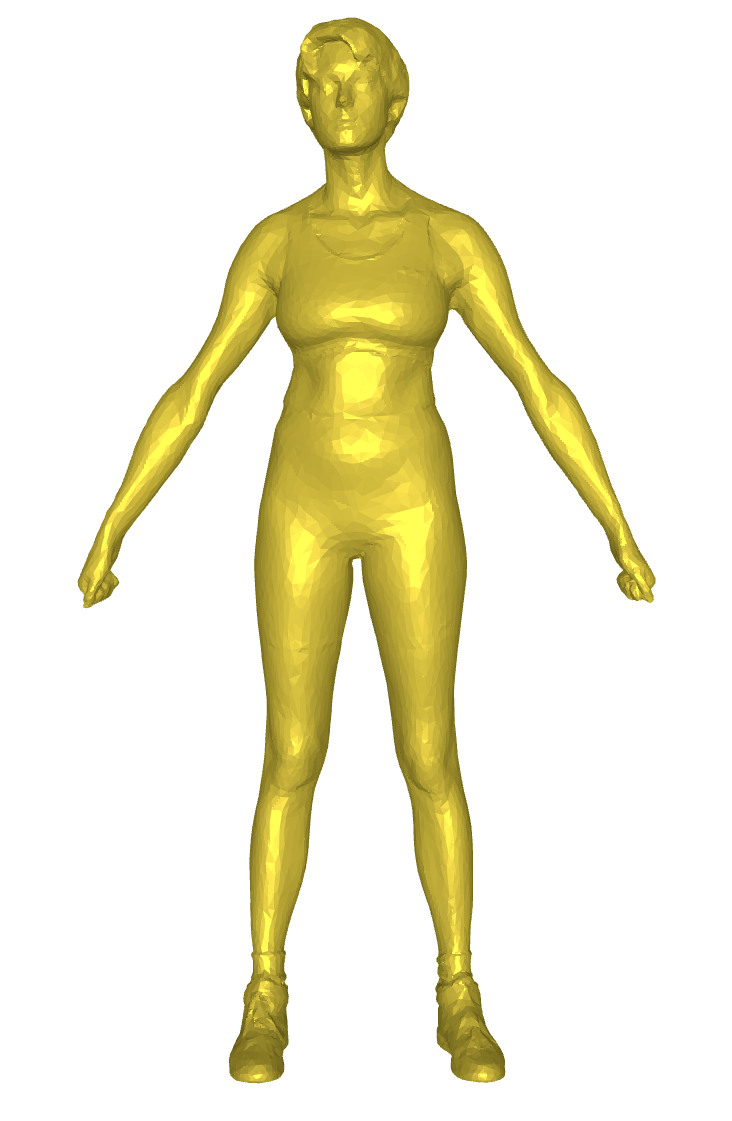
\includegraphics[width=.3\textwidth]{./human3d.png}\hfill
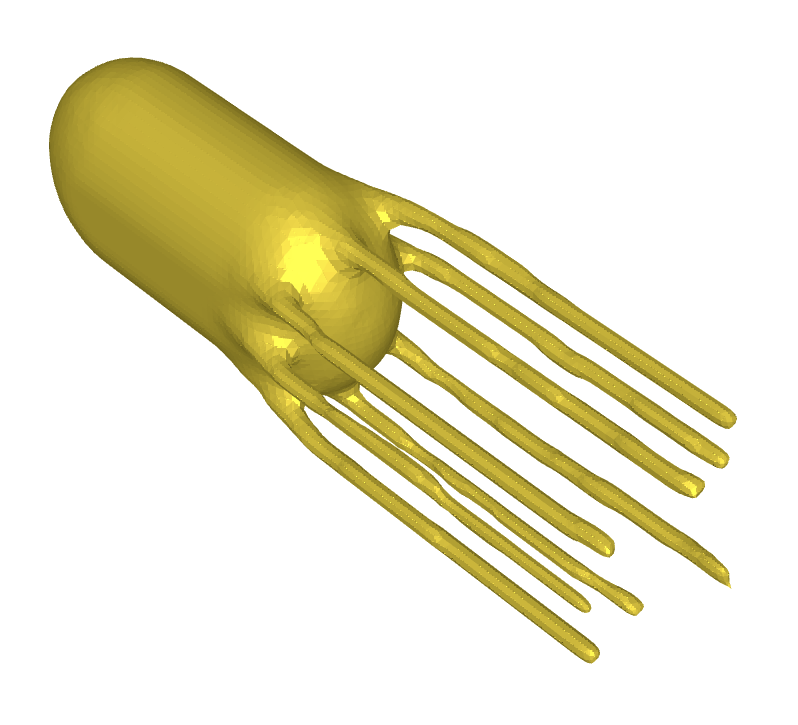
\includegraphics[width=.3\textwidth]{./octopus3d.png}\hfill
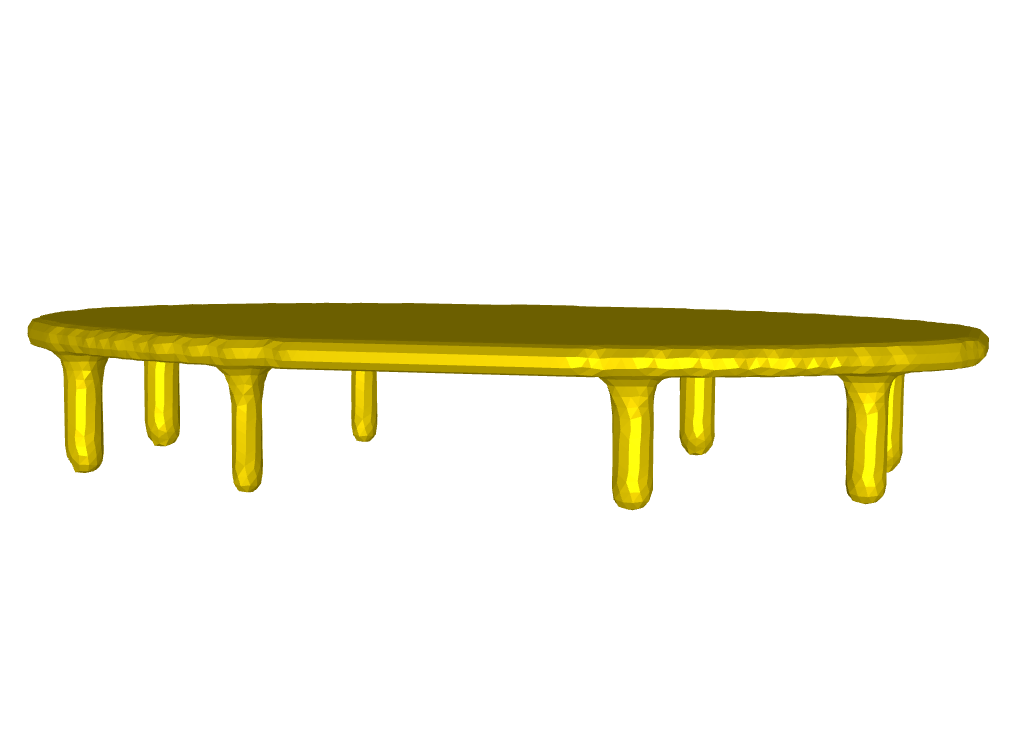
\includegraphics[width=.3\textwidth]{./table3d.png}

\caption{Meshes of 3-dimensional point clouds representing from left to right: a human, an octopus and a table.}
\label{fig:3d_shape}
\end{figure}



\begin{figure}[H]

\centering
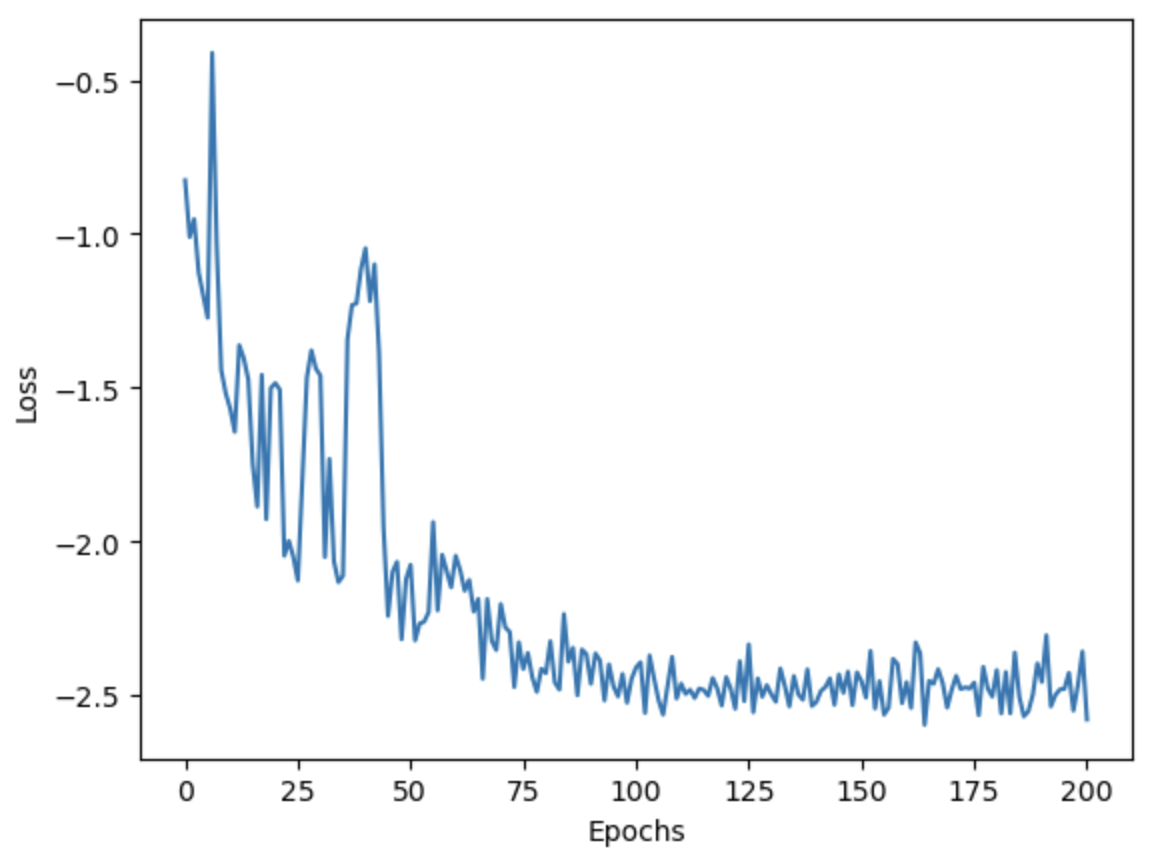
\includegraphics[width=.3\textwidth]{./human_curve.png}\hfill
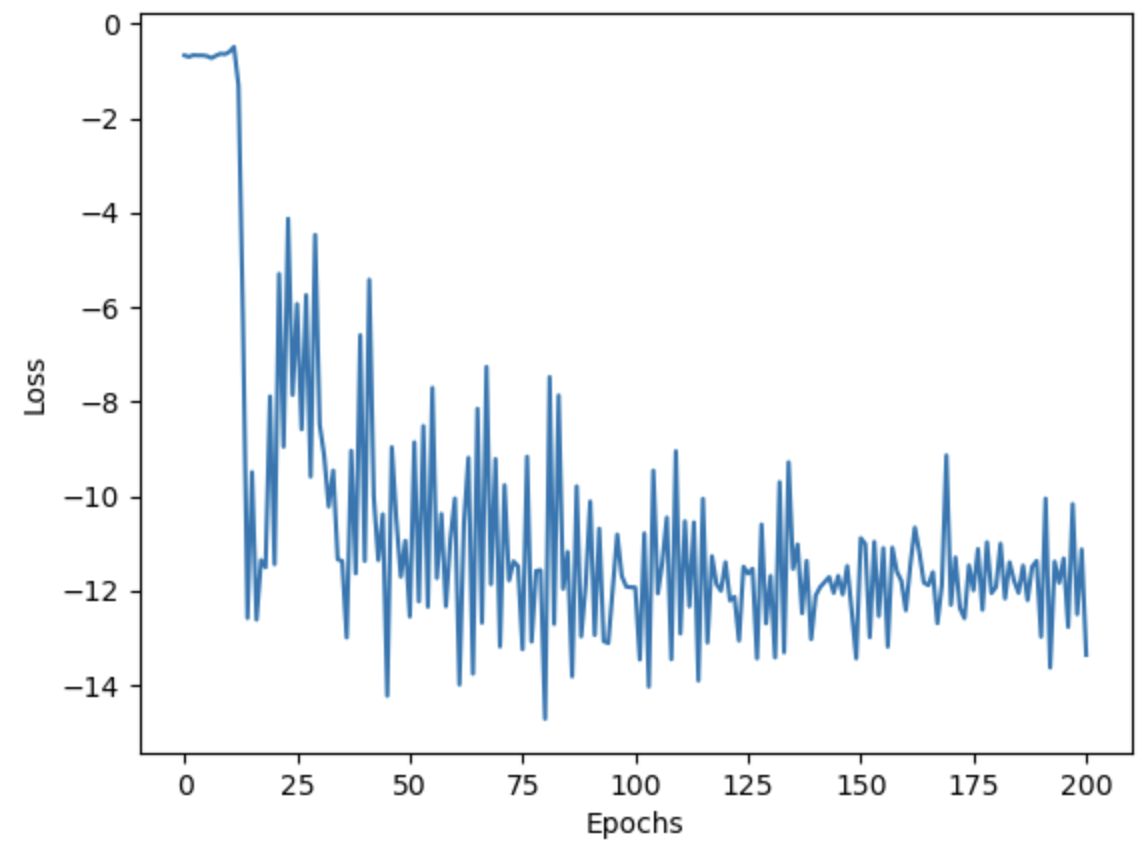
\includegraphics[width=.3\textwidth]{./octopus_curve.png}\hfill
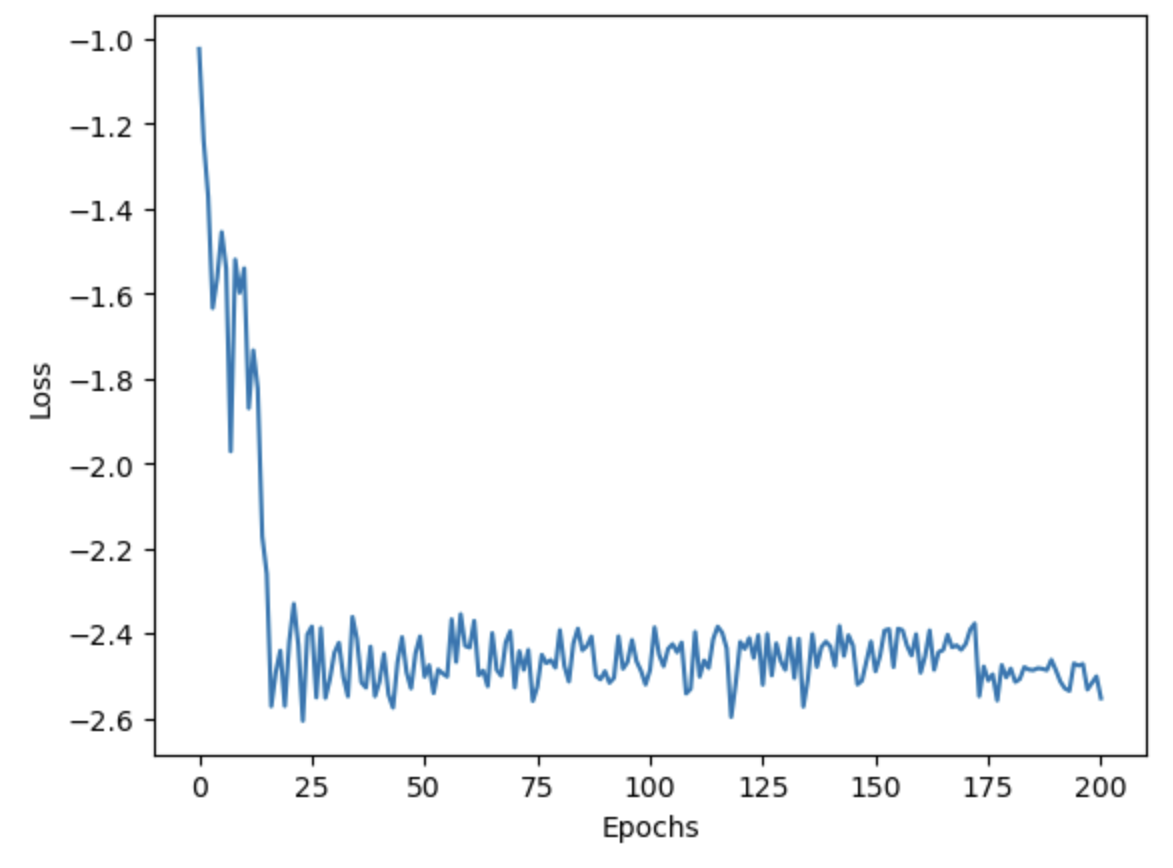
\includegraphics[width=.3\textwidth]{./table_curve.png}

\caption{Learning curves for the 3-dimensional shapes corresponding, from left to right, to: the human, the octopus and the table.}
\label{fig:3d_curves}

\end{figure}

\begin{table}[H]
    \centering
    \begin{tabular}{|c|c|c|}
    \hline
     Human    &  Octopus & Table\\
     \hline
     0.9999    & -0.9984 & 0.9993\\
     \hline
    \end{tabular}
    \caption{Correlation between the optimized directions and the optimal ones, for each 3-dimensional shape.}
    \label{tab:3d_correlations}
\end{table}

\begin{figure}[H]

\centering
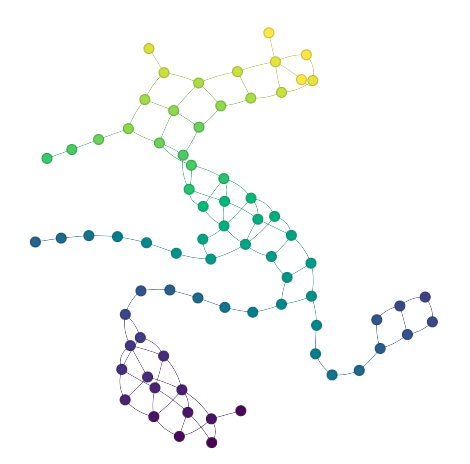
\includegraphics[width=.3\textwidth]{./human_initial.png}\hfill
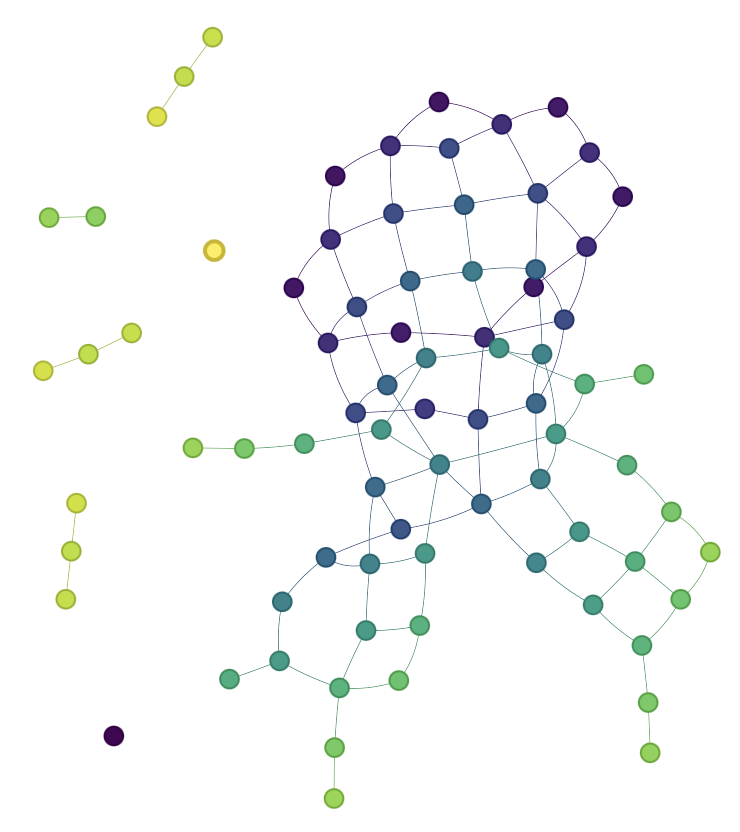
\includegraphics[width=.3\textwidth]{./octopus_initial.png}\hfill
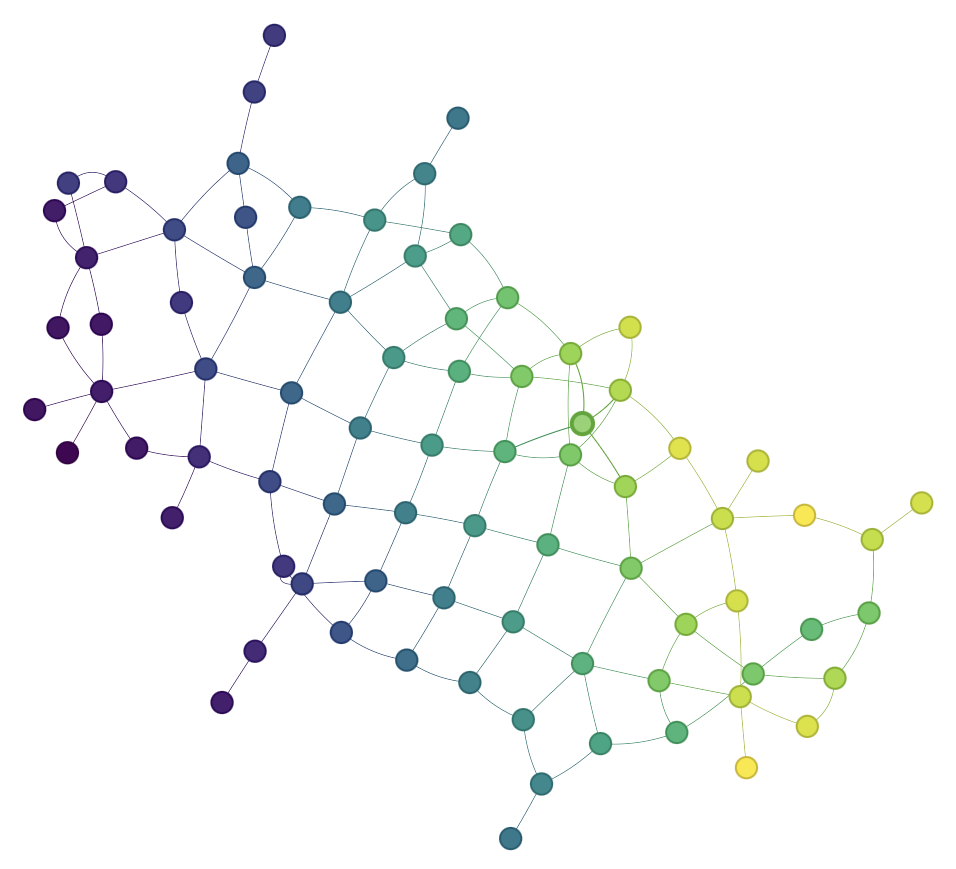
\includegraphics[width=.3\textwidth]{./table_initial.png}

\caption{Regular Mapper graphs computed with the initial filter function, corresponding, from left to right, to: the human, the octopus and the table. Vertices are colored using the mean value of the filter function in the corresponding clusters.}
\label{fig:3d_initial}

\end{figure}

\begin{figure}[H]

\centering
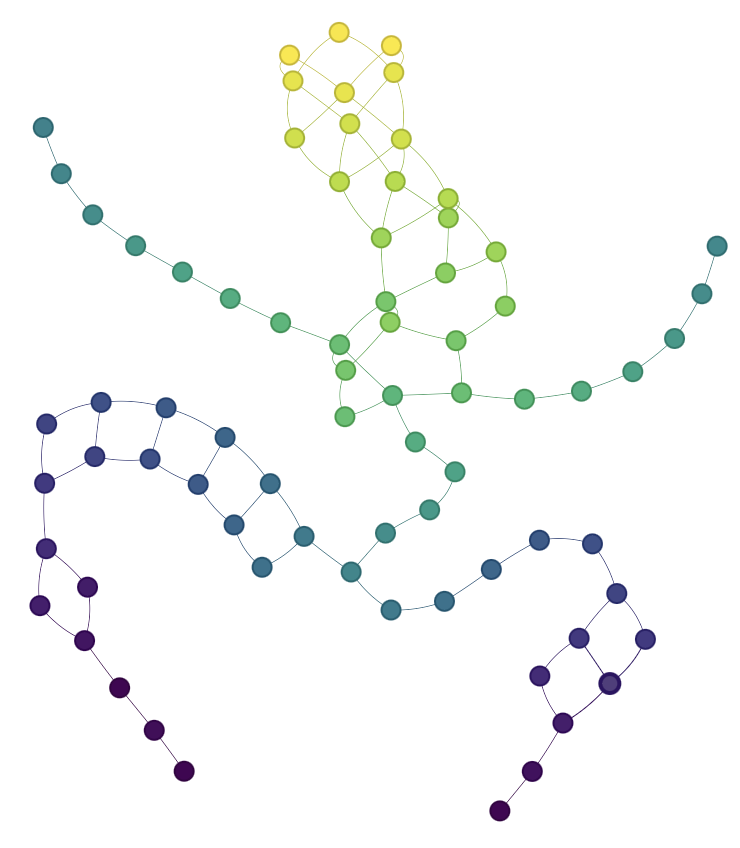
\includegraphics[width=.3\textwidth]{./human_final.png}\hfill
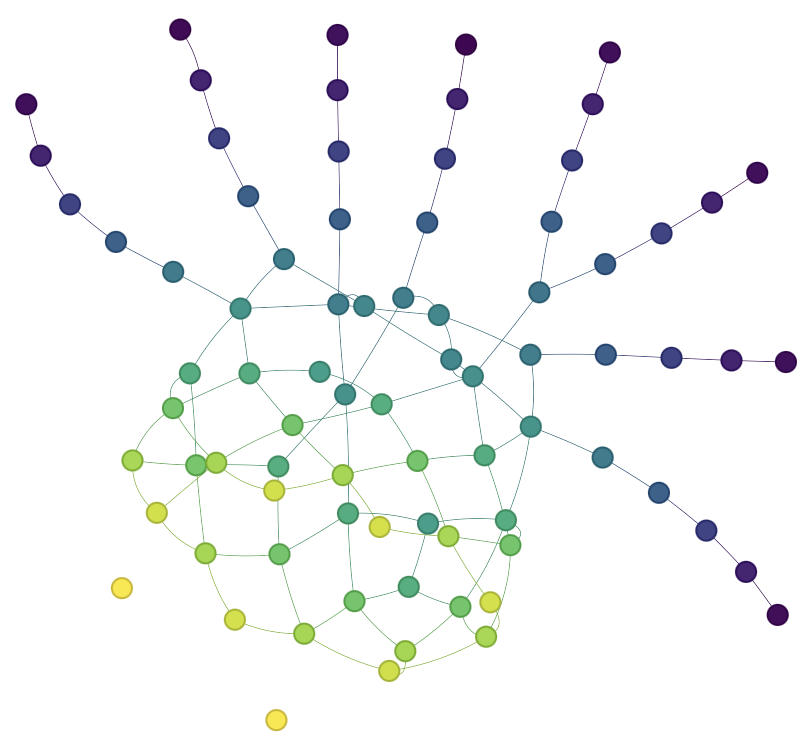
\includegraphics[width=.3\textwidth]{./octopus_final.png}\hfill
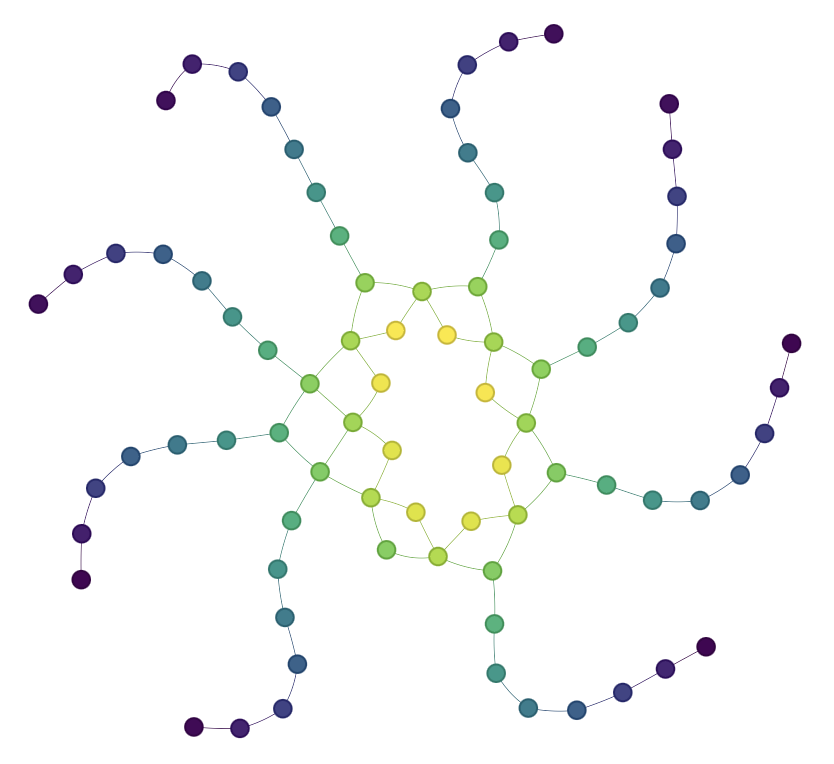
\includegraphics[width=.3\textwidth]{./table_final.png}

\caption{Regular Mapper graphs computed with the optimized filter function, corresponding, from left to right, to: the human, the octopus and the table. Vertices are colored using the mean value of the filter function in the corresponding clusters.}
\label{fig:3d_final}

\end{figure} 



\subsection{Mapper optimization on RNA-sequencing data}
\label{subsec:single-cell}


%\paragraph*{Human preimplantation dataset.}
We now apply Mapper optimization on the human preimplantation dataset of \cite{petropoulos2016single}, which can also be found in the tutorial of the \texttt{scTDA} Python library. The dataset consists of $n=1,529$ cells form $88$ human preimplantation embryos, sampled at $5$ different timepoints. The dataset can be accessed in the following link \cite{sctda}, and it contains the expression levels for $p=26,270$ genes for each individual cell. The information of the sampling timepoint for each cell is also given, but we do not include it during optimization. The dataset is first preprocessed using the \texttt{Seurat} package in \texttt{R} (gene counts for each cell are divided by the total counts for that cell and multiplied by $10^4$, and then they are natural-log transformed using $\log(1+\cdot)$), which produces a normalized dataset $\Xs_n\subseteq\mathbb{R}^p$.
The parametric family of filter functions we wish to optimize is also linear here, i.e. equal to $\{f_\theta\colon x\mapsto\langle x,\theta \rangle,\,\theta\in\mathbb{R}^p\}$, and the cover assignment scheme $A_\delta$ is the smooth relaxation of the standard case with $\delta=10^{-5}\cdot(\max_{x\in\Xs_n}f_\theta(x)-\min_{x\in\Xs_n}f_\theta(x))$. The cover of the image space is given by $25$ intervals of the same length, such that consecutive intervals have a percentage of $30\%$ of their length in common. The clustering algorithm used is agglomerative clustering and its threshold is fixed using a Hausdorff distance heuristic: we first compute the Hausdorff distance between $\Xs_n$ and a randomly sampled subset of $\Xs_n$ of size $ n/3\approx500$, then we manually tune the threshold using factors of this distance until we get Mapper graphs of reasonable size.

\paragraph*{Objective.} To find $\bar\theta$, we use the total extended persistence as a persistence specific loss $\loss$ and we run Algorithm \ref{alg1} with $N=200$ and $M=10$, taking the diagonal as the initial direction, i.e. $\theta_0=(\frac{1}{\sqrt{p}},...,\frac{1}{\sqrt{p}})^T$. The learning curve in displayed in Figure \ref{fig:sctda_curve} of Appendix~\ref{apdx:experiments}.
The regular Mapper graphs computed using the initial and the final filter functions are displayed in Figure \ref{fig:sctda_mappers}, and are colored with respect to the time component (which was not included in the training dataset).

\begin{figure}[H]
    \centering
    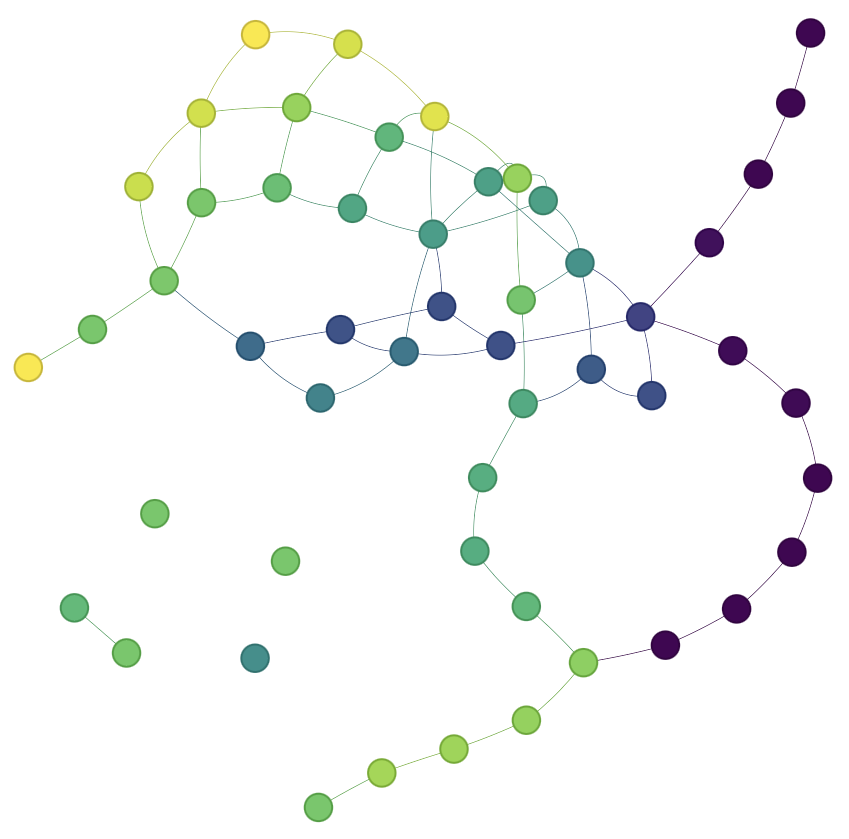
\includegraphics[width=.3\textwidth]{./sctda_initial.png}\hspace{0.05\textwidth}
    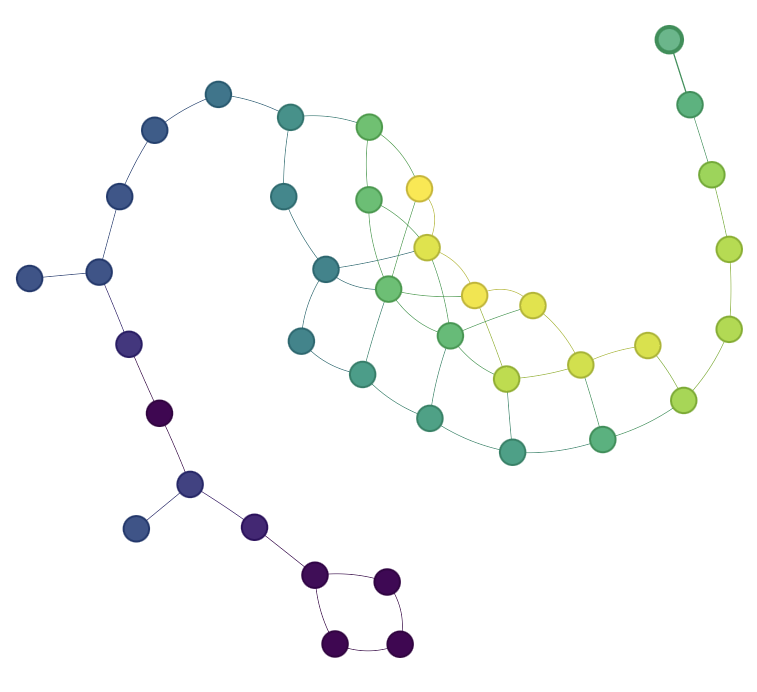
\includegraphics[width=.3\textwidth]{./sctda_final.png}
    \caption{Regular Mapper graphs for the human preimplantation dataset computed using: in the left the initial filter function and in the right the optimized filter function. Vertices are colored using the mean value of the sampling timepoint in the clusters.}
    \label{fig:sctda_mappers}
\end{figure}


\paragraph*{Qualitative assessment.} One can see that the data representation in the Mapper graph produced by the optimized filter function fits the time structure better than with the initial function. In order to confirm this, we isolate each subset of cells having the same sampling timepoint and we plot their respective estimated densities with respect to the initial and the optimized filter function values, in Figure \ref{fig:sctda_densities}. One can see that the optimized filter that we captured is capable of sorting the cells with respect to time, especially at the early timepoints. The reduced performance in this aspect for the later timepoints is, in our guess, due to slowing down of the cell differentiation process. Furthermore, the comparison, in Table \ref{tab:sctda_pearsonr} of Appendix~\ref{apdx:experiments}, between Pearson's correlation coefficients also show that the optimized filter is more correlated to time. \\
%In \cite{rizvi2017single}, a Mapper graph built on the same dataset, where the filters are the first two PCA components, is used. To extract a pseudo-time from the Mapper graph, correlations, between the time and graph distances defined on the different nodes, are first computed. This requires prior knowledge of the time component, whereas our approach uses only the gene expression matrix.
We also verify that the branches in our optimized Mapper graph correspond to the same two genes, HTR3E for the early timepoints and CDX1 for the later ones, that were identified by \cite{rizvi2017single}, see Figure \ref{fig:sctda_genes}. We also identified a few nodes in the branch containing the cells which were sampled in the early stages, that do not contain a high expression level for the HTR3E gene. This could potentially point out another subpopulation of cells with distinct genomic profiles, and that our optimized Mapper graph has captured. An additional experiment using single cell RNA-sequencing data is given in Appendix \ref{apdx:mef}.
 
\begin{figure}[H]
    \centering
    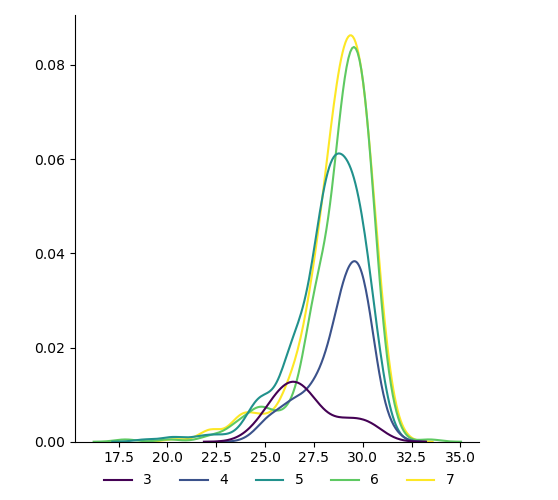
\includegraphics[width=.3\textwidth]{./sctda_densities_initial.png}
    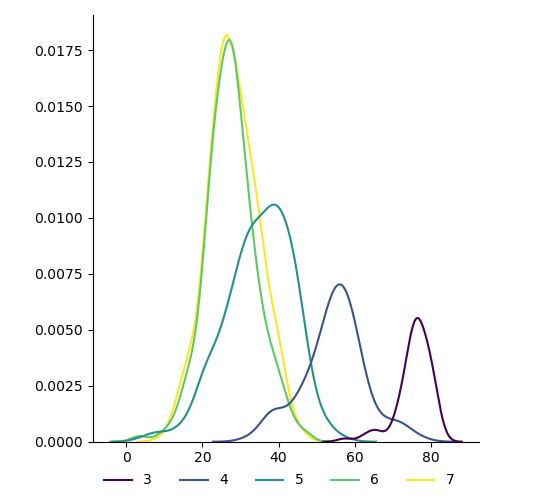
\includegraphics[width=.3\textwidth]{./sctda_densities_final.png}
    \caption{Estimated density of each subset of cells having the same sampling timepoint, with respect to: in the left the initial filter function values and in the right the optimized filter function values. Colors indicate the sampling timepoint in days.}
    \label{fig:sctda_densities}
\end{figure}
 
\begin{figure}[H]
    \centering
    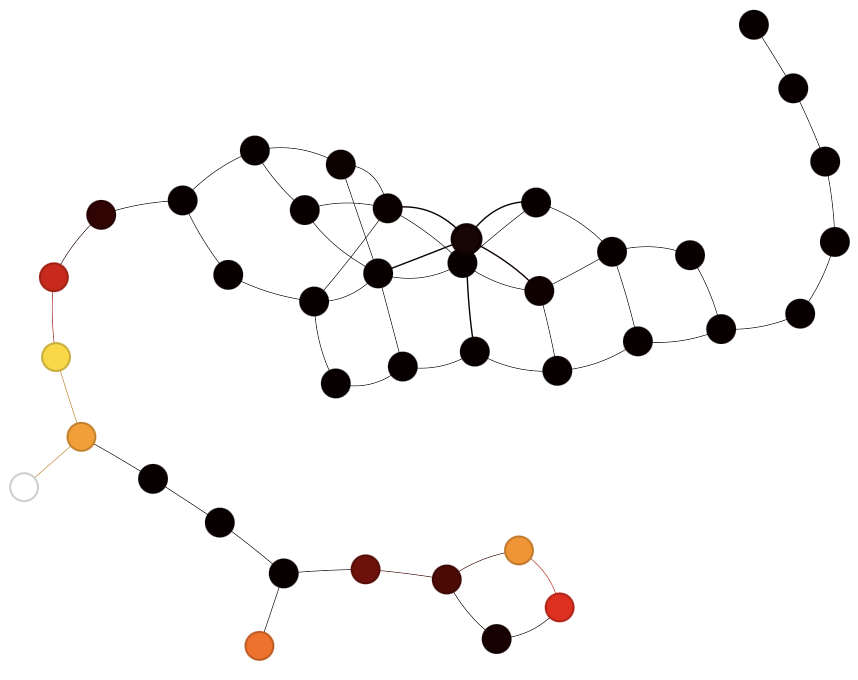
\includegraphics[width=.3\textwidth]{./sctda_htr3e.png}\hspace{0.05\textwidth}
    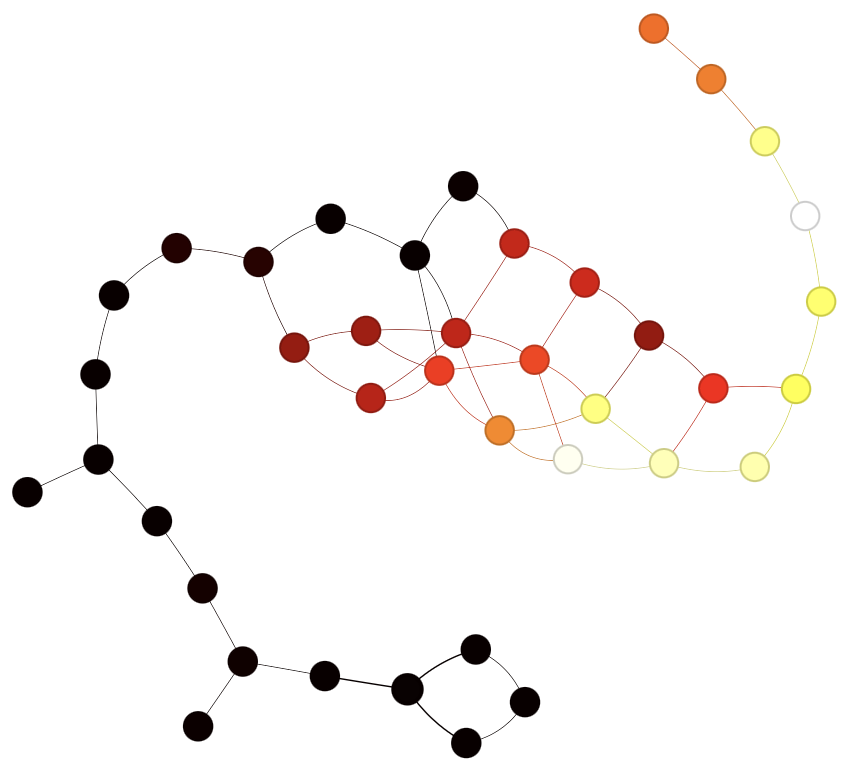
\includegraphics[width=.3\textwidth]{./sctda_cdx1.png}
    \caption{Regular Mapper graph computed using the optimized filter function, colored using the mean normalized expression of: in the left gene HTR3E and in the right gene CDX1.}
    \label{fig:sctda_genes}
\end{figure}

